\section{Training Dynamics of RLVR}
\label{sec:training_analysis}

To further demystify RLVR, we reproduce and analyze the training recipe of DAPO~\citep{yu2025DAPO-Zero}, which has been demonstrated to present extended reasoning capability boundaries in Section~\ref{sec:benchmark_analysis}. Our experiments show that its training dynamics align pretty well with Theorem~\ref{thm:grpo-incentive}.

%TODO: move this earlier?
\paragraph{Key Indicators}
We first introduce key indicators that we have recorded during the reproduction.
For each prompt $q$ sampled with $G$ responses, we define the number of answer passes and the number of both CoT and answer passes as $C = \sum_{i=1}^G \mathcal{I}_{\text{Ans}}(a_i)$ and $D = \sum_{i=1}^G \mathcal{I}_{\text{CoT}}(c_i) \cdot \mathcal{I}_{\text{Ans}}(a_i)$, respectively.
We follow~\citet{chen2021CodeX}'s approach to calculate the Pass@K metric.
Accordingly, we have per-prompt metrics: $\text{Pass@K}^{(q)} = 1 - \frac{\binom{G - C}{K}}{\binom{G}{K}} $ and $\text{CoT-Pass@K}^{(q)} = 1 - \frac{\binom{G - D}{K}}{\binom{G}{K}}$.
Besides, we estimate the probability of producing correct answers for prompt $q$ as $P(CA)^{(q)} = \frac{C}{G}$ and the probability of producing correct CoTs when generating correct answers as $P(CC|CA)^{(q)} = \frac{D}{C}$.
For a dataset of multiple prompts, we take an average of per-prompt metrics as the dataset-level score.

\begin{figure*}[t]
\centering
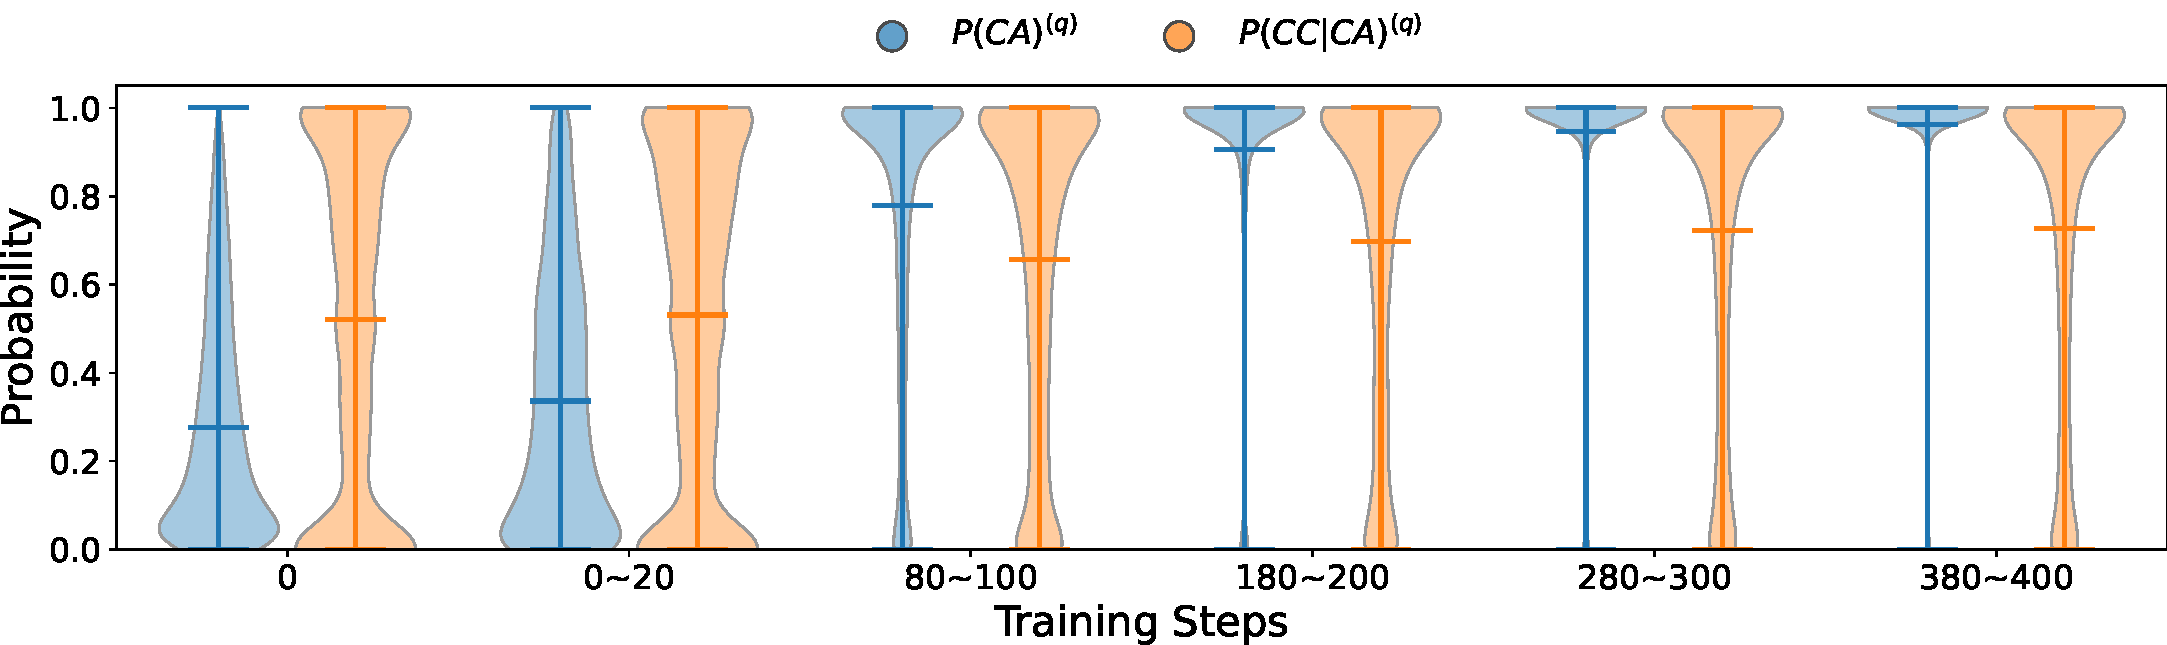
\includegraphics[width=0.95\linewidth]{figures/rollout_verify_easy.pdf}
\caption{
The evolution of $P(CA)^{(q)}$ (the fraction of correct answers for prompt $q$) and $P(CC|CA)^{(q)}$ (the fraction of correct CoTs within the correct answers for prompt $q$) for fully optimized training questions over the course of DAPO training.
}
\label{fig:q_ca_cc_in_training}
\end{figure*}

\begin{figure*}[t]
\centering
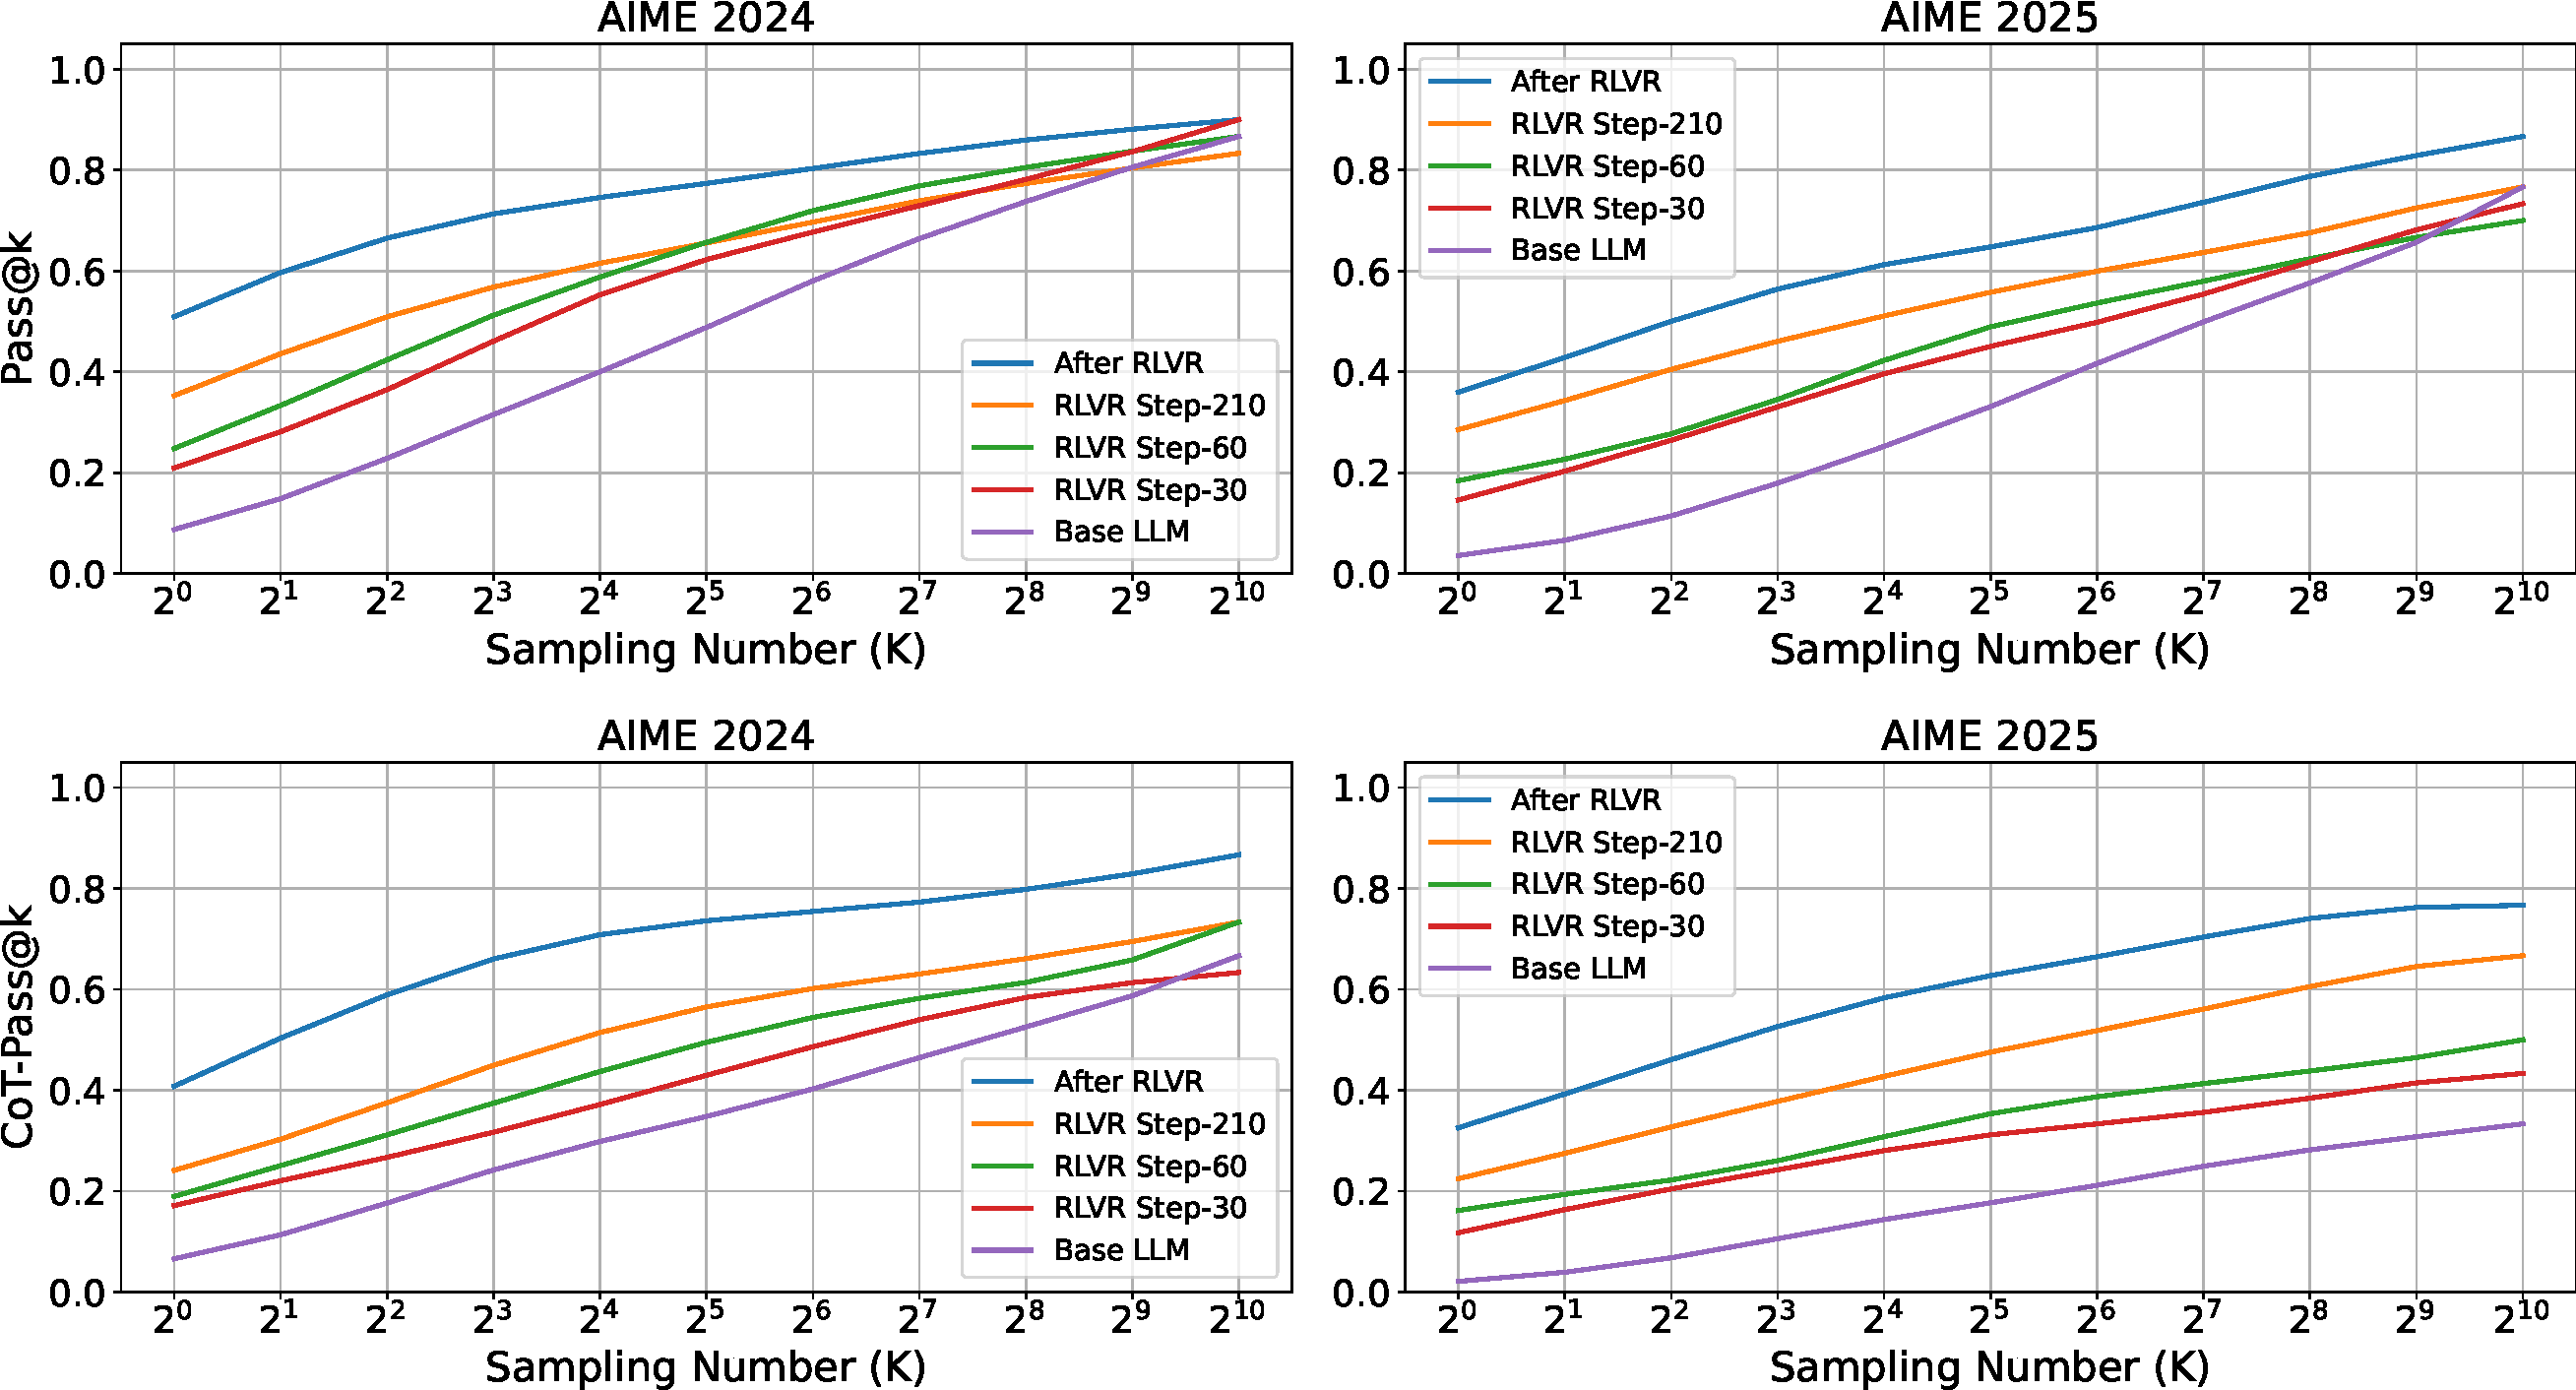
\includegraphics[width=0.95\textwidth]{figures/rl_process_aime_passk.pdf}
\caption{
The evolution of Pass@K (the top row) and CoT-Pass@K (the bottom row) performance on AIME 2024 and 2025 for different model checkpoints during the DAPO training.
}
\label{fig:eval_training_ckpts}
\end{figure*}

\paragraph{Optimization Effects}
In our reproduced DAPO training, we observe that most training questions have been fully optimized.
As shown in Figure~\ref{fig:q_ca_cc_in_training}, the probability of generating correct answers for these questions almost reach $1$.
In the meanwhile, we also observe the improvement in producing more correct reasoning CoTs, as indicated by the improvements in $P(CC|CA)^{(q)}$.
These observations validate the key perspective in Theorem~\ref{thm:grpo-incentive}: RLVR not only optimizes the final verifiable reward but also implicitly incentivizes correct reasoning.

\paragraph{Generalization Behaviors}
In the meanwhile, Figure~\ref{fig:eval_training_ckpts} discloses that the optimization of RLVR leads to the generalization improvements of both Pass@K and CoT-Pass@K from the very beginning.
And using the CoT-Pass@K metric, we can clearly tell that the reasoning capability boundary has also been enhanced since the beginning.
Another interpretation for this empirical observation is that the model has learned to produce more and more reasoning CoTs that DeepSeek-R1-0528-Qwen-8B cannot identify any error.
This ability is learned implicitly since we have no formal supervision for the CoT correctness.

\paragraph{Limitations of DAPO}
Figure~\ref{fig:q_ca_cc_in_training} also unveils the limitations of DAPO, the R1-zero approach applied to a 32B base LLM.
As $P(CA)^{(q)}$ approaches $1.0$ for most fully optimized training questions after 400 steps, which means these questions are no longer learnable because we cannot calculate a valid GRPO advantage for a all-correct group, we can still observe a non-negligible portion of imperfect CoTs (the median of $P(CC|CA)^{(q)}$ is around $0.7$).
These signals indicate that there are certain unexpected reasoning behaviors learned in DAPO and we may not have a chance to mitigate them purely based on answer correctness as the reward.